\documentclass[11pt]{article}
\usepackage[margin=0.5in]{geometry}
\usepackage{todonotes}
\usepackage{natbib}
\usepackage{graphicx}
\usepackage{listings}
\usepackage{color}
\usepackage{hyperref}
\usepackage{multirow}
\usepackage{pifont}
\usepackage{xcolor,colortbl}
\usepackage{hyperref}
\hypersetup{colorlinks=true,linkcolor=black,citecolor=blue,filecolor=black,urlcolor=blue}
\usepackage{amsmath}
 
\newcommand{\tristan}[1]{\color{orange}\textbf{From Tristan:}#1\color{black}}
\newcommand{\Yohan}[1]{\todo[inline,backgroundcolor=green]{YC:#1}}
\newcommand{\cross}[0]{\cellcolor{red!65}\ding{53}}
\newcommand{\valid}[0]{\cellcolor{green!75!black}\ding{51}}
\newcommand{\warn}[0]{\cellcolor{orange!75}?}

\lstdefinestyle{customPython}{
  belowcaptionskip=1\baselineskip,
  breaklines=true,
  xleftmargin=\parindent,
  language=Python,
  showstringspaces=false,
  basicstyle=\scriptsize\ttfamily,
  keywordstyle=\bfseries\color[rgb]{0.580, 0.000, 0.827},
  %{purple!40!lightgray},
  commentstyle=\itshape\color{green!40!black},
  identifierstyle=\bfseries\color{cyan!75!black},
  stringstyle=\color{orange},
  deletekeywords={double,float},
  classoffset=1, % starting new class
  otherkeywords={double,float},
  morekeywords={double,float},
  keywordstyle=\bfseries\color{green!55!black},
  classoffset=0
}


\begin{document}

\title{PyTracer: Automatically profiling numerical instabilities in Python}
\author{Yohan Chatelain$^1$, Gregory Kiar$^2$, Nigel Young$^1$, Tristan Glatard$^1$\\
$^1$Department of Computer Science and Software Engineering, Concordia University, Montreal, Canada\\
$^2$Center for the Developing Brain, Child Mind Institute, New York, NY, USA}
\date{}
\maketitle

\begin{abstract}
[abstract goes here]
\end{abstract}

\section{Introduction}

The scientific Python ecosystem is a central ingredient of scientific
analyses due to its rich offering of data manipulation, array programming,
numerical analysis, and visualization tools. In particular, libraries such
as NumPy~\cite{harris2020array}, SciPy~\cite{virtanen2020scipy}, scikit-learn~\cite{pedregosa2011scikit} or PyTorch~\cite{paszke2019pytorch} are used in hundreds of publications every year, providing a reference set of high-quality open-source core scientific libraries. Numerous domain-specific data analysis pipelines were built from this ecosystem by diverse research groups, leveraging Python's simplicity and expressivity. 

Numerical stability is a crucial requirement of reliable scientific data
processing. In unstable analyses, tiny numerical perturbations introduced
by data noise, software and hardware updates, or parallelization lead to
substantial deviations in final results and potentially different scientific conclusions, threatening the reliability of computational analyses. To address this issue, numerical stability analyses need to be conducted systematically. However, no practical tool currently exists to conduct such analyses on Python programs.

We present PyTracer, a numerical stability analyzer for Python programs.
PyTracer adopts a dynamic approach that evaluates numerical stability using program execution traces, allowing scaling to large programs without manual intervention. In contrast, theoretical approaches based on condition number or backward error analyses require detailed modelling of the program and its numerical implementation. Similarly, static code analysis techniques such as Frama-C~\cite{cuoq2012frama}, Gappa~\cite{de2010certifying} or Flocq~\cite{boldo2011flocq} hardly scale to large codebases, particularly in dynamically-typed languages such as Python.

PyTracer estimates the significant digits of Python floating-point variables by combining program traces obtained with different numerical perturbations, which requires (1) tracing floating-point computations along program executions, (2) generating numerically-perturbed executions, and (3) visualizing stability evaluations. PyTracer addresses these requirements with (1) dynamic instrumentation of Python functions, modules and classes through meta-programming, (2) a ``fuzzy" Python interpreter instrumented with Monte-Carlo arithmetic, and (3) an interactive Plotly dashboard to visualize stability measures throughout program executions.

Through stability evaluations of 
SciPy, scikit-learn, and pyAFQ~\cite{kruper2021evaluating} --- an analysis toolbox for diffusion magnetic resonance imaging --- we demonstrate PyTracer as a practical solution to review the numerical stability of extensive code bases. The remainder of this manuscript describes related approaches, presents the design of PyTracer, and demonstrates its potential on various use cases.

% \begin{itemize}
%     \item Numerical instabilities are inherent to numerical computations \tristan{not only to HPC, also software updates, small perturbations in parameters or data}
%     \item 
%     \item Neuroimaging tools are facing reproducibility issues, one factor of which is numerical stability \tristan{neuroimaging should be an illustration, your intro should rather focus on Python in general, it's much more impactful} 
%     \item Detecting those instabilities is challenging: large data sets, large pipeline, long computation time, complex physics \tristan{Here you could illustrate the point with neuroimaging pipelines}
%     \item Needs tools for automatically detecting these instabilities
%     \item Needs tools to quickly identify unstable functions among large number of calls
% \end{itemize}

\section{Related work}

In this section, we review tools and theoretical frameworks related to Pytracer components.
We start by reviewing state-of-the-art dynamic tools for detecting numerical instabilities.
Then, we focus on existing theoretical approaches for perturbations-based techniques to detect numerical instabilities,
Pytracer being agnostic to perturbation technique used. Finally, we review visualization tools 
aiming at detecting numerical instabilities over execution time.

\label{sec:soa}
\subsection{Numerical assessment tools}

Several tools have been and continue to be developed to assess numerical quality.
Those tools can be divided in two main categories: static VS dynamic analysis.
Static analysis focuses on safety and soundness of error bounds provided 
while dynamic analysis rather provides proof-less numerical quality estimations.
The main drawback of static analysis tools is the poor scalability that confine them to small programs.
Pytracer falls into the second category by targeting real Python use cases.
In this section, we will hence review the most known tools based on dynamic analysis.
We divide the tools in three sections starting by tools dedicated to non Python codes, then 
tools using Dynamic Binary Instrumentation and finally tools dedicated to Python codes.

Following the languages mainly used in HPC or embedded systems, 
most the tools are dedicated to C, C++ or FORTRAN codes. 
Those tools are either source-to-source or compiler based transformations.
CADNA~\cite{jezequel2008cadna} is a library for C, C++ and Fortran codes implementing
the CESTAC~\cite{vignes1993stochastic} method, a stochastic arithmetic used for detecting round-off
errors by introducing numerical instabilities in floating-point computations.
Verificarlo~\cite{verificarlo} is a compiler that instruments floating point operations
to replace them by generic call to Verificarlo API, providing several backends implementations including one for 
Monte Carlo Arithmetic (MCA) (cf.~\ref{sec:mca}), another stochastic arithmetic.
Bao et al. ~\cite{bao2013fly} modifies gcc to track local floating-point error across execution.
pLiner~\cite{guo2020pliner} is root cause analyzer based upon clang that detects floating point operations 
responsible of result variability. 
It uses source-to-source transformation at AST level to rewrite parts of code with higher precision and to compare the result with
the original one. PFPSanatizer~\cite{chowdhary2021parallel} is a compiler that uses parallel shadow execution to detect numerical issues
by using higher precision. 
Shaman~\cite{demeure_phd} is a C++ library that uses a first-order error model to propagate numerical error. 
FLiT~\cite{sawaya2017flit} is framework to detect variability induced by compilers and their optimizations.
Tang et al.~\cite{tang2016software} propose a source-to-source framework for executing targeted code 
in infinite and fixed precision with and without using stochastic arithmetic.

The main other existing approach uses Dynamic Binary Instrumentation (DBI) to perform analysis at the binary level,
removing the language barrier and allowing to analyze any binary without needing the source code. This approach
is particularly relevant on closed-source software. However, working at binary level loses high-level information useful
for debugging and understanding the source code semantic and logic.
CraftHPC~\cite{lam2013dynamic} uses DBI to detect catastrophic cancellations at runtime.
Verrou~\cite{fevotte2016verrou} is a Valgrind~\cite{nethercote2007valgrind} based tool that replaces on-the-fly
floating-point operations by their stochastic arithmetic counterparts. FPDebug~\cite{benz2012dynamic} uses DBI to detect numerical 
inaccuracies by using shadow computations with a higher precision.
Herbgring~\cite{sanchez2017finding} is a Valgrind-based tool to detect
numerical instabilities. It uses a shadow memory to do detect precision losses by comparison with results obtained with the high-precision 
MPFR library~\cite{fousse2007mpfr}. It is combined with symbolic computation to backtrack the root of the error.

Existing tools for tracing Python code are dedicated to performance profiling, for time (cProfile) 
or memory consumption (memprofile). 
To the best of our knowledge, there is currently no tool dedicated to numerical analysis.
We can nevertheless mention Anteater~\cite{faust2019anteater} a Python tracer tool that aims at debugging Python application. 
It operates source transformation at AST level but only deals with native numeric Python types.
However, we can compare the methodology used by these tools against the one used in Pytracer.
These tools use an instrumentation based on decorators, a Python mechanism allowing 
to wrap a function by adding a line over a function declaration.
While this method is useful when targeting specific functions, it becomes time consuming 
when applied to a large number of functions since one need to tag functions by hand,
which clearly not tractable for large codes like numpy. Moreover, the user has most of the time no clues
about where numerical instability comes from and must therefore all functions as potentially suspect. 
This issue enforces the need to use automatic approaches.
It's worth mentioning that DBI based tools can be used for Python because they are language agnostic but
they are not intended to analyze Python code and do not take into account high-level information about 
types being used or detailed stack trace. Moreover, few tools embed a visualizer for 
analyzing numerical quality over time letting the postprocessing to the user. 

\tristan{The content of this section is excellent but the structure is a bit messy. Would you like to restructure in 3 paragraphs as follows? (1) There's no numerical instrumentation tools in Python (your last paragraph + anteater), (2) DBI tools could be used but won't provide a detailed stack trace, (3) tools for other languages.}

\subsection{Detecting instabilities}

We review here the existing theoretical framework that might be used to detect numerical instabilities.


\label{sec:mca}
\subsubsection{Monte Carlo Arithmetic}
\tristan{Add a sentence to connect this part to the previous one. Something like: We use Monte-Carlo arithmetic to detect numerical instabilities. You could also summarize what the other options would be.} \tristan{cite \cite{parker1997monte}}

MCA simulates round-off errors by introducing random perturbations in floating point computations. Each floating point number is replaced by its MCA counterparts:
\[
inexact(x) =  x + \beta^{e_x - t}\xi
\]
where $\beta$ is the basis, $t$ the virtual precision and $\xi \in (-\frac{1}{2},\frac{1}{2})$ a random variable.
Virtual precision is one strength of the MCA method since it allows simulating 
reduced working precision.
MCA comes with three modes: Random Rounding (RR), Precision Bounding (PB) and FullMCA where either the output, either the inputs or both are perturbed with the $inexact$ function.
While the RR mode is equivalent to stochastic rounding, PB mode allows identifying 
catastrophic cancellations.

MCA provides a formula to compute the number of significant digits:
\[
s = -\log_{\beta}{ \left| \dfrac{\sigma}{\mu} \right|}
\]
where $\sigma$ and $\mu$ are respectively the empirical standard deviation and expected value of a variable $x$ evaluating several times with MCA. 
Note that this formula gives an approximation of the real $s$ and 
one can refer to~\cite{sohier2018confidence} to obtain associated rigorous confidence intervals.

\subsection{Visualization}

SHAMAN, CADNATrace;
Veritracer~\cite{chatelain2018veritracer} is an extension of Verificarlo~\cite{verificarlo} that aims 
at visualizing the numerical stability over time for C, C++ and Fortran codes.

\section{PyTracer design}

% \subsection{Pytracer workflow}

PyTracer follows a three step approach. First, selected functions are automatically
instrumented before executing the targeted application. During the execution, instrumented
functions will dump their inputs and outputs in a file called a trace. 
The idea is to profile several times the application to measure discrepancies between runs.
Based on the set of traces obtained from multiple executions, Pytracer 
will gather them into one trace containing statistics about each traced variables.
With all information gathered, the user can visualize and interact with it through a Ploty/Dash server.

\begin{figure}
    \centering
    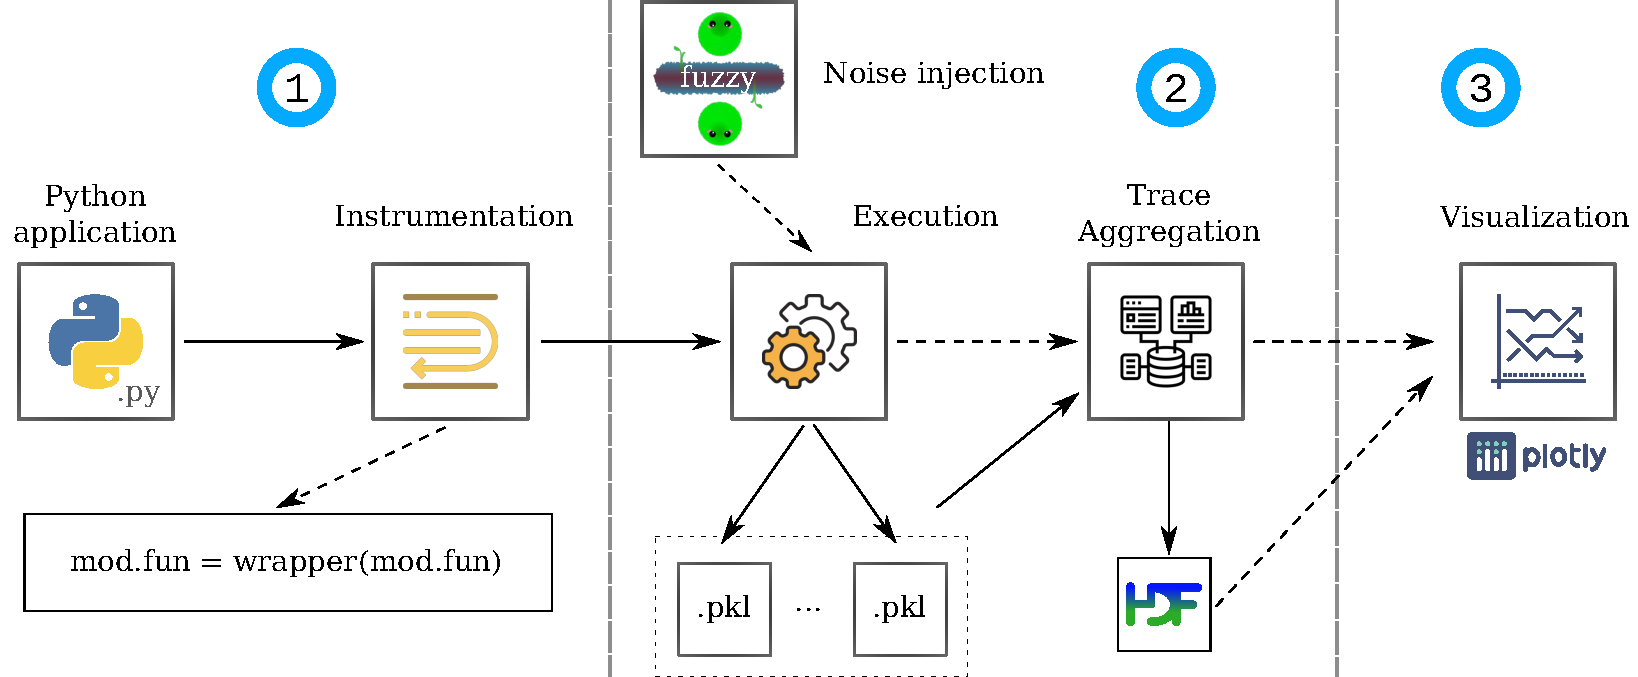
\includegraphics[width=\linewidth]{figure/workflow.pdf}
    \caption{Pytracer workflow \tristan{Excellent figure but fuzzy should appear}}
    \label{fig:workflow}
\end{figure}

\subsection{Instrumentation}

Pytracer dynamically instruments the Python modules selected by the user
without requiring modifications of the targeted application.
To do so, Pytracer creates a new version of each selected module 
by preserving the attributes' signature, allowing to use them
transparently in the original application.
If by default Pytracer instruments all attributes present
in a given module, except the special attributes of the form \texttt{\_\_*\_\_},
the wrapping is not always be feasible as detailed in section ?.
The original attributes are then preserved and the user is warned.
The user can also restrict the list of attributes to trace through
a mechanism of inclusion/exclusion. 

The main advantage of this method is its transparency for the user
since this latter only needs to select which modules to trace and Pytracer instrument them for him.
Moreover, the code does not need to be changed contrary to the method based on decorators, allowing
to use instrument functions when the source code is not available or editable, like for instance
in singularity containers or when running on HPC cluster.

\subsection{Module import interception}

Modules in Python are loaded through the import mechanism by the \texttt{import} keyword.
During this process, Python is looking for module path file in the default system paths and those provided by
the user (with \texttt{PYTHONPATH}). When the selected module is found, Python executes it for triggering 
instructions in the \texttt{\_\_init\_\_.py} file and stores it in the \texttt{sys.modules} map,
acting as a cache. 

Pytracer intercepts the module loaded by using the \texttt{Finder} and \texttt{Loader} mechanism.
The Finder is responsible for finding the loader for a module that is being imported while the 
Loader loads and initializes the module. We add a new Finder and Loader on top of the default ones
to intercept imports and to wrap modules selected by the user. This mechanism allows returning 
the original module in the wrapper code and returning the wrapped one in the targeted application
without modifying the actual code.

\subsubsection{Module functions}

The module function is the simplest case to deal with.
For each function encountered in a module, Pytracer
creates a wrapper around this function that is dynamically compiled with the \textit{compile}
builtin function. The original function is then replaced by its wrapped counterpart.

However, this technique cannot be applied for all functions, especially for 
callable instances, which are instances of class that can be called like traditional functions
but that contain attributes. Indeed, using a wrapper would 1) modify the type of the instance
that could cause semantic bugs 2) hide attributes that causes \texttt{AttributeError} exceptions.

\begin{figure}
    \centering
\begin{lstlisting}[language=Python,style=customPython]
def getwrapperfunction(function_module, function_name, function, function_wrapper_name):
    function_wrapper_name = f
    function_id = id(function)
    info = (function_id, function_module, function_name)
    wrapper_code = f"""
    def {function_wrapper_name}(*args, **kwargs):
        return generic_wrapper({info},*args,**kwargs)"""
    return wrapper_code
\end{lstlisting}
    \caption{Caption}
    \label{fig:wrapper_code}
\end{figure}

\subsubsection{Classes}

Overriding Python classes is similar to module functions.
Pytracer goes through the attributes and replaces each callable attribute (method) by its wrapped counterpart.
The resulting class has the same type as the original one, avoiding type conflicts.
However, some classes forbid overwriting attributes of their instances, in particular the `\_\_call\_\_` operator
allowing to call an instance as a function.
Moreover, no general solution can be provided since some Python classes are non-inheritable 
like \texttt{bool},\texttt{NoneType} or \textit{universal functions} in numpy (\texttt{ufunc})
and thus cannot be inherited to overload operators.
The solution consisting in replacing function by a wrapper cannot be applied here.

This issue was mostly encountered with numpy ufunc that are intensively used in numpy. Universal functions are vectorized element-wise operators on
multidimensional arrays (\texttt{ndarrays}). They are implemented in C code with target specialized versions to achieve best performance.
One should then implement subclassing mechanism in C, which is contrary to Pytracer philosophy to be as non-intrusive and portable as possible.
However, since \texttt{ufunc} are intensively used in scientific computational codes (elementary mathematical functions are ufunc in numpy),
we implement a special treatment for them. Numpy provides the \texttt{frompyfunc} helper function to create \texttt{ufunc} from arbitrary function.
The main problem with this approach is that the output type is \texttt{PyObject} representing abstract object that conflicts 
when used as index. Figure illustrates this issue. As a last resort, user may disable \texttt{ufunc} tracing by Pytracer.


\begin{figure*}
\begin{minipage}[t]{0.4\linewidth}
    \begin{lstlisting}[language=Python,style=customPython]
>>> import numpy as np
>>> x = np.array(range(10))
>>> index = np.array([1,-1],dtype=int)
>>> x[index]
>>> array([1, 9])
    \end{lstlisting}
    \label{fig:wrapper_code}
\end{minipage}
\begin{minipage}[t]{0.4\linewidth}
    \begin{lstlisting}[language=Python,style=customPython]
>>> import numpy as np
>>> x = np.array(range(10))
>>> index = np.array([1,-1], dtype=object)
>>> x[index]
Traceback (most recent call last):
  File "<stdin>", line 1, in <module>
IndexError: arrays used as indices must be of integer (or boolean) type
    \end{lstlisting}
    \label{fig:wrapper_code}
\end{minipage}
\caption{Illustration of the issue of using \texttt{frompyfunc} function to convert function to \texttt{ufunc}.}
\end{figure*}

\subsection{Detecting instabilities}

\subsubsection{Fuzzy environment}

We use the fuzzy~\cite{kiar2020comparing} environment to use MCA in Python.
The fuzzy ecosystem provides a Python interpreter recompiled with Verificarlo.
Verificarlo~\cite{verificarlo} is a compiler based upon clang~\cite{lattner2008llvm}
that replaces all floating-point operations by a generic call. 
The user can then link these generic calls with different floating-point models 
(called backends) during the execution. Verificarlo proposes several 
backends~\cite{chatelain2019automatic,chatelain2019outils} including for MCA.

The main advantage of the fuzzy ecosystem is its transparency for the user.
One can directly use its python code with the fuzzy python interpreter
without manual interventions. Moreover, the fuzzy ecosystem is intended to be
modular by providing fuzzy version of numpy, scipy and scikit-learn modules.
One can thus choose the fuzzy stack desired.

\subsection{Interactively visualization}

\subsubsection{Plotly}

\begin{figure}
    \centering
    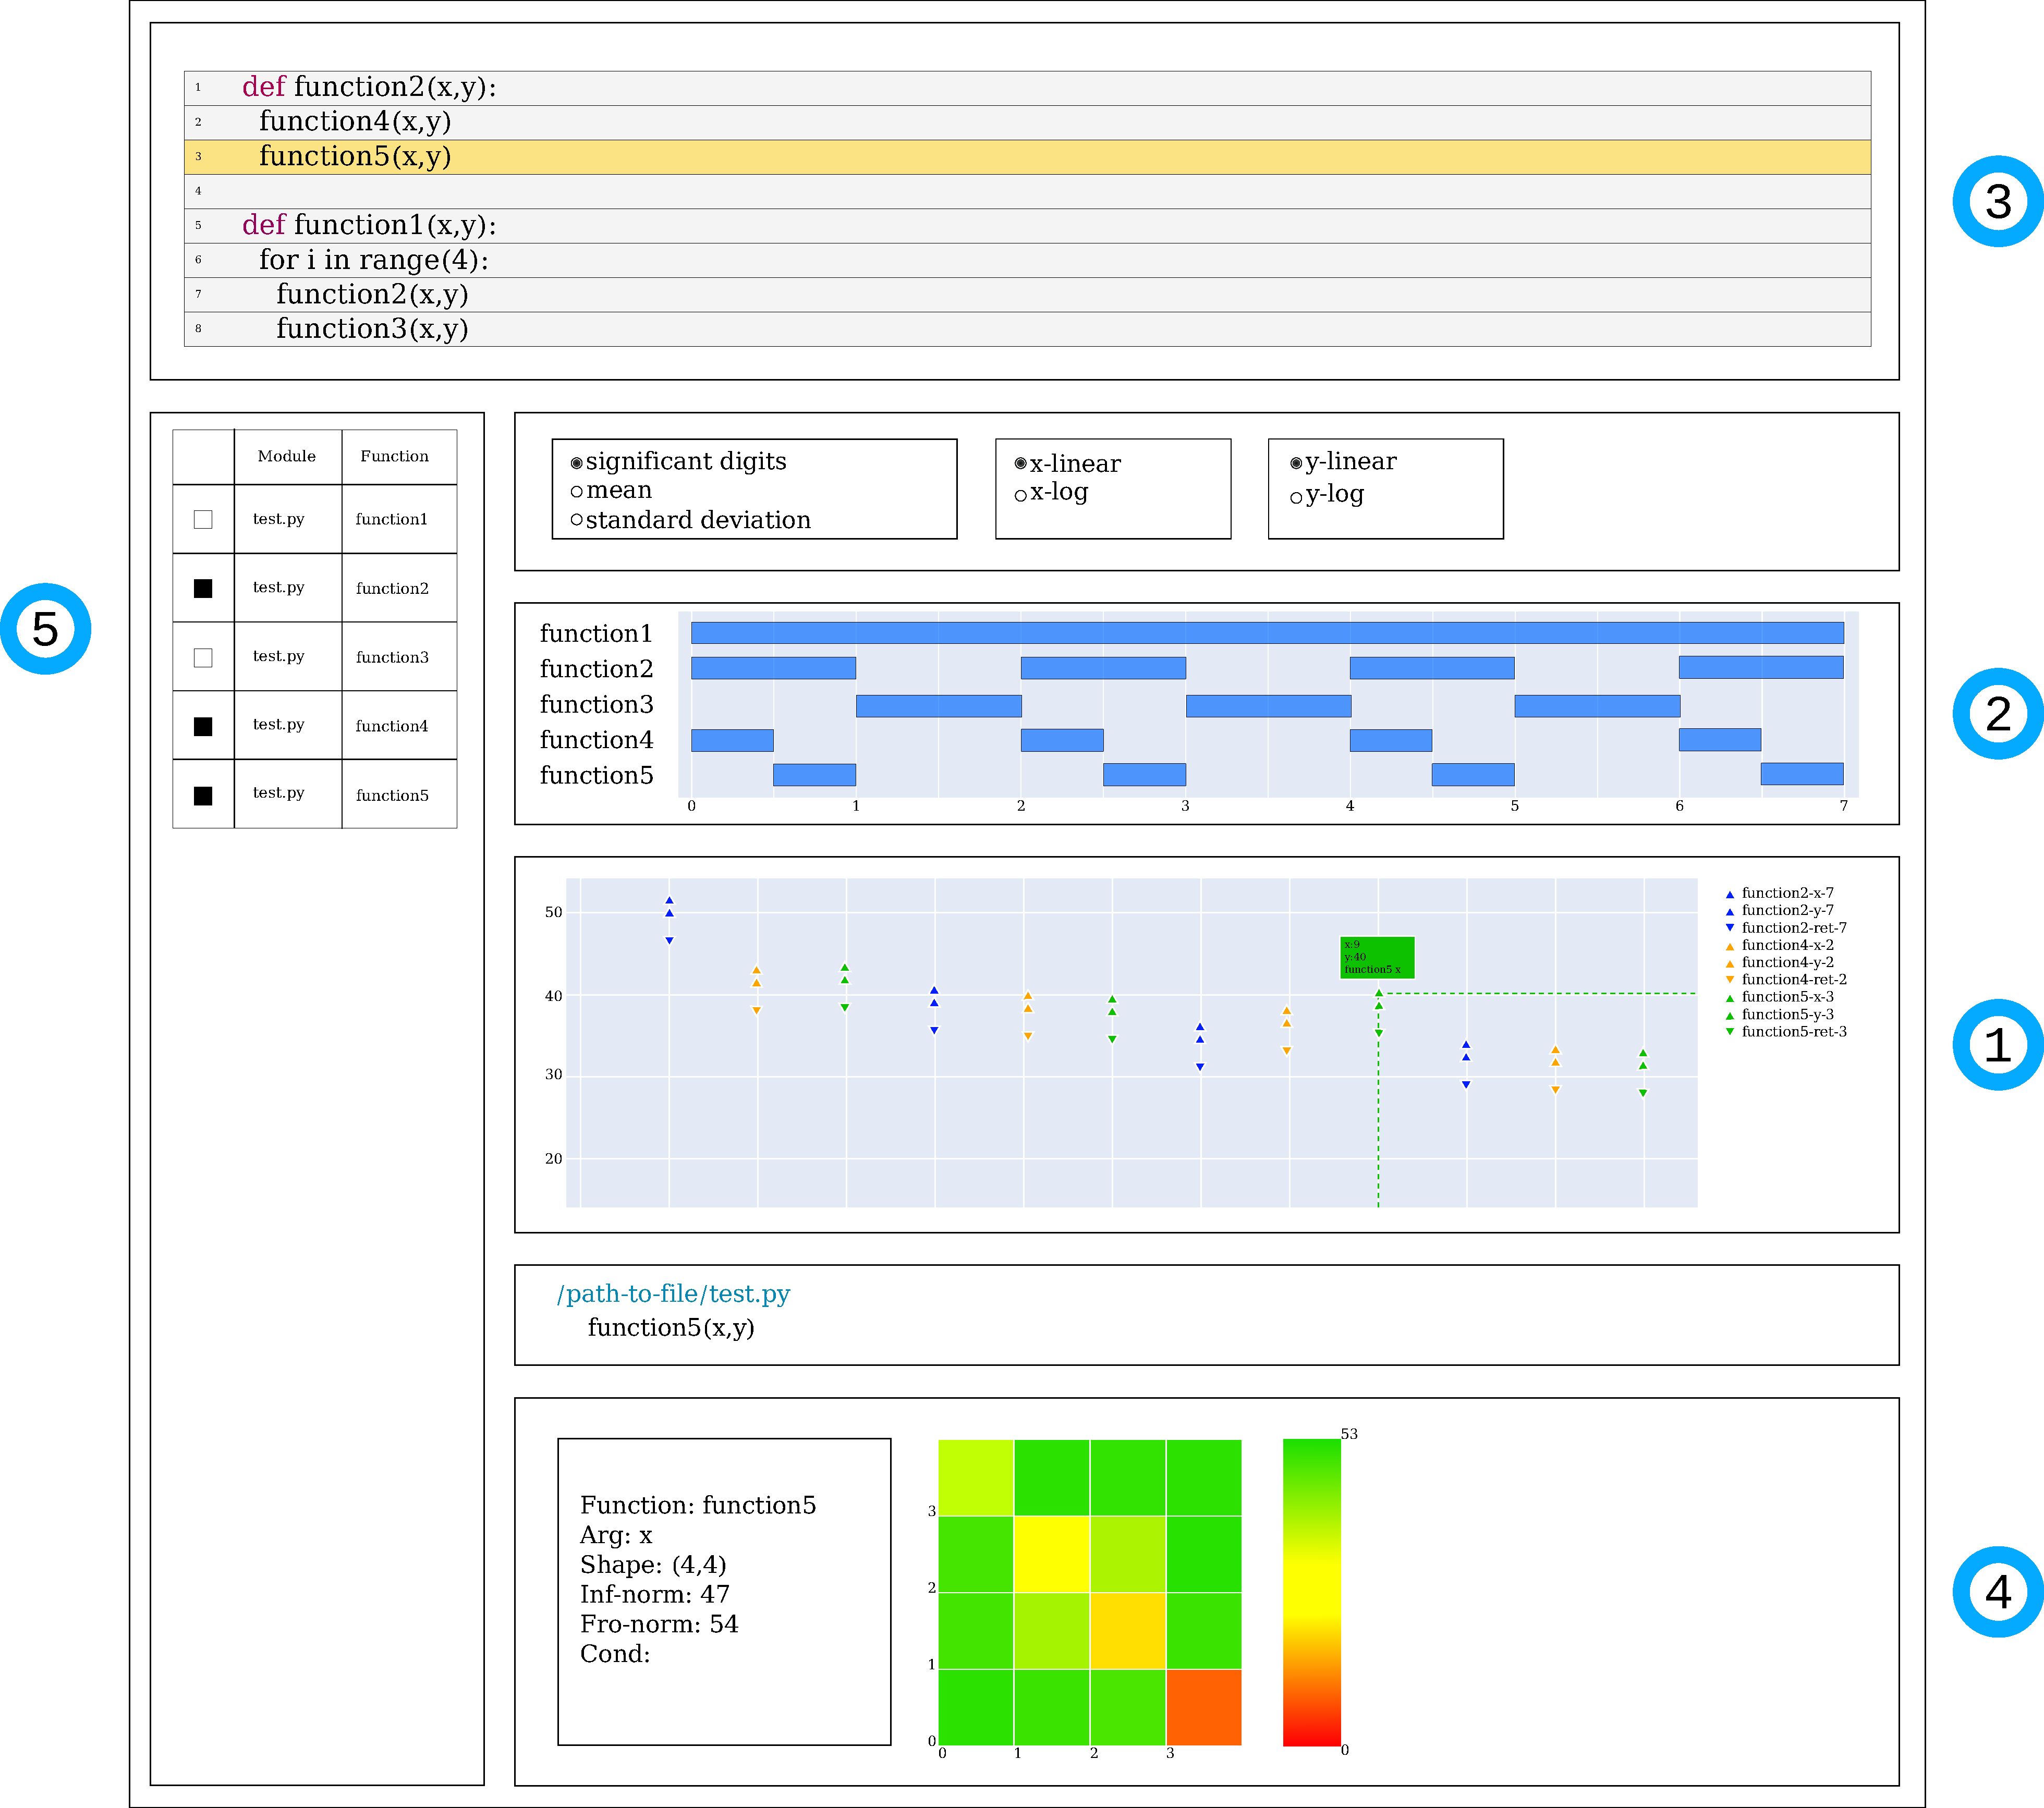
\includegraphics[width=\linewidth]{figure/pytracer_layout.pdf}
    \caption{Pytracer visualization layout.}
    \label{fig:my_label}
\end{figure}



\section{Use cases}

\subsection{SciPy}

We tested Pytracer on SciPy~\cite{virtanen2020scipy} examples provided in the Tutorial website section.
SciPy is organized in several libraries targeting specific computing domains.
We focused on the following packages:
\begin{itemize}
    \item \texttt{fftpack}: Fast Fourier Transform routines
    \item \texttt{interpolate}: Interpolation and smoothing splines
    \item \texttt{optimize}: Optimization and root-finding routines
    \item \texttt{integration}: Integration and ordinary differential equation solvers
\end{itemize}

% \begin{table}[]
%     \centering
%     \begin{tabular}{|c|c|c|c|c||c|c|c|c|}
%     \hline
%     \multirow{3}{5em}{Application} & \multicolumn{4}{|c||}{RR} & \multicolumn{4}{|c|}{MCA} \\\cline{2-9}
%                 & \multicolumn{2}{|c|}{numpy} &  \multicolumn{2}{|c||}{no numpy} & \multicolumn{2}{|c|}{numpy} & \multicolumn{2}{|c|}{no numpy} \\\cline{2-9}
%                 & run & parse &  run & parse & run & parse & run & parse \\
%     \hline
%     %        &               RR                 &                 MCA               \\
%     %        &  numpy         &   no numpy      &      numpy      &     no numpy    \\
%     %        & run   & parse  &  run   &  parse &  run   & parse  & run    & parse  \\
%     \multirow{4}{5em}{Interpolate}
%     \multirow{12}{5em}{Optimize}
%     \multirow{3}{5em}{FFT}
%     Adaboost & \warn & \valid & \valid & \valid & \warn & \cross & \cross & \cross \\
%     Bayesian Ridge Regression & \warn & \valid & \valid & \valid & \cross & \cross & \cross & \cross \\
%     Online classifier comparison & \valid & \valid & \valid & \valid & \cross & \cross & \cross & \cross  \\
%     Cluster Iris & \valid & \valid & \valid & \valid & \valid & \cross & \valid & \cross \\
%     Covariance estimation & \valid & \cross & \valid & \cross & \cross & \cross & \valid & \cross \\
%     Decision Tree Regression & \valid & \valid & \valid & \valid & \valid & \cross & \valid & \cross \\
%     Digits Classification & \warn & \valid & \valid & \valid & \warn & \cross & \cross & \cross \\
%     Face Recognition & \cross & \valid & \cross & \valid & \cross & \cross & \cross & \cross \\
%     L1 Penalty & \warn & \valid & \valid & \valid & \warn & \cross & \valid & \valid \\
%     Lasso and elastic net & \warn & \valid & \valid & \valid & \warn & \cross & \valid & \cross \\
%     Separating hyperplan & \valid & \valid & \valid & \valid & \valid & \cross & \valid & \cross \\
%     MNIST classification & \warn & \valid & \valid & \valid & \valid & \cross & \valid & \valid \\
%     Multitask Lasso & \warn & \valid & \valid & \valid & \warn & \cross & \valid & \valid \\
%     Orthogonal matching & \warn & \valid & \valid & \valid & \cross & \valid & \cross & \valid \\
%     PCA decomposition & \warn & \valid & \valid & \valid & \warn & \cross & \valid & \cross \\
%     Robust Linear Regression & \valid & \valid & \valid & \valid & \warn & \cross & \valid & \cross \\
%     Segmentation toy & \warn & \valid & \valid & \cross & \warn & \cross & \cross & \cross \\
%     SVM & \valid & \valid & \valid & \valid & \valid & \cross & \valid & \cross \\
%     Tomography & \warn & \valid & \valid & \cross & \warn & \cross & \cross & \cross \\
%     Weighted samples & \valid & \valid & \valid & \valid & \valid & \cross & \valid & \cross \\
%     \hline
%     \end{tabular}
%     \caption{Pytracer executions summary}
%     \label{tab:pytracer_sklearn_results_summary}
% \end{table}

\subsection{Scikit learn}

We tested Pytracer on Scikit-learn~\cite{pedregosa2011scikit}, a "Python module integrating a wide range of state-of-the-art machine learning algorithms for medium-scale supervised and unsupervised problems".
Scikit-learn offers a well supplied and documented list of examples that facilitates its using with Pytracer.
Among the several available examples, we choose the following representative set:
\href{https://scikit-learn.org/stable/auto_examples/ensemble/plot_adaboost_regression.html#sphx-glr-auto-examples-ensemble-plot-adaboost-regression-py}{Decision Tree Regression with AdaBoost},
\href{https://scikit-learn.org/stable/auto_examples/linear_model/plot_bayesian_ridge.html#sphx-glr-auto-examples-linear-model-plot-bayesian-ridge-py}{Bayesian Ridge Regression}, 
\href{https://scikit-learn.org/stable/auto_examples/linear_model/plot_sgd_comparison.html#sphx-glr-auto-examples-linear-model-plot-sgd-comparison-py}{Comparing various online solvers}, 
\href{https://scikit-learn.org/stable/auto_examples/linear_model/plot_sgd_comparison.html#sphx-glr-auto-examples-linear-model-plot-sgd-comparison-py}{K-means Clustering},
\href{https://scikit-learn.org/stable/auto_examples/linear_model/plot_sgd_comparison.html#sphx-glr-auto-examples-linear-model-plot-sgd-comparison-py}{Recognizing hand-written digits},
\href{https://scikit-learn.org/stable/auto_examples/decomposition/plot_faces_decomposition.html#sphx-glr-auto-examples-decomposition-plot-faces-decomposition-py}{Faces dataset decompositions},
\href{https://scikit-learn.org/stable/auto_examples/linear_model/plot_logistic_l1_l2_sparsity.html#sphx-glr-auto-examples-linear-model-plot-logistic-l1-l2-sparsity-py}{L1 Penalty and Sparsity in Logistic Regression},
\href{https://scikit-learn.org/stable/auto_examples/linear_model/plot_lasso_and_elasticnet.html#sphx-glr-auto-examples-linear-model-plot-lasso-and-elasticnet-py}{Lasso and Elastic Net for Sparse Signals},
\href{https://scikit-learn.org/stable/auto_examples/linear_model/plot_sgd_separating_hyperplane.html#sphx-glr-auto-examples-linear-model-plot-sgd-separating-hyperplane-py}{SGD: Maximum margin separating hyperplane},
\href{https://scikit-learn.org/stable/auto_examples/linear_model/plot_sparse_logistic_regression_mnist.html#sphx-glr-auto-examples-linear-model-plot-sparse-logistic-regression-mnist-py}{MNIST classification using multinomial logistic + L1},
\href{https://scikit-learn.org/stable/auto_examples/linear_model/plot_sgd_iris.html#sphx-glr-auto-examples-linear-model-plot-sgd-iris-py}{Plot multi-class SGD on the iris dataset},
\href{https://scikit-learn.org/stable/auto_examples/linear_model/plot_multi_task_lasso_support.html#sphx-glr-auto-examples-linear-model-plot-multi-task-lasso-support-py}{Joint feature selection with multi-task Lasso},
\href{https://scikit-learn.org/stable/auto_examples/linear_model/plot_omp.html#sphx-glr-auto-examples-linear-model-plot-omp-py}{Orthogonal Matching Pursuit},
\href{https://scikit-learn.org/stable/auto_examples/decomposition/plot_pca_iris.html#sphx-glr-auto-examples-decomposition-plot-pca-iris-py}{PCA example with Iris Data-set},
\href{https://scikit-learn.org/stable/auto_examples/linear_model/plot_poisson_regression_non_normal_loss.html#sphx-glr-auto-examples-linear-model-plot-poisson-regression-non-normal-loss-py}{Poisson regression and non-normal loss},
\href{https://scikit-learn.org/stable/auto_examples/cluster/plot_segmentation_toy.html#sphx-glr-auto-examples-cluster-plot-segmentation-toy-py}{Spectral clustering for image segmentation},
\href{https://scikit-learn.org/stable/auto_examples/svm/plot_separating_hyperplane_unbalanced.html#sphx-glr-auto-examples-svm-plot-separating-hyperplane-unbalanced-py}{SVM: Separating hyperplane for unbalanced classes},
\href{https://scikit-learn.org/stable/auto_examples/applications/plot_tomography_l1_reconstruction.html#sphx-glr-auto-examples-applications-plot-tomography-l1-reconstruction-py}{Compressive sensing: tomography reconstruction with L1 prior (Lasso)},
\href{https://scikit-learn.org/stable/auto_examples/linear_model/plot_tweedie_regression_insurance_claims.html#sphx-glr-auto-examples-linear-model-plot-tweedie-regression-insurance-claims-py}{Tweedie regression on insurance claims},
\href{https://scikit-learn.org/stable/auto_examples/linear_model/plot_sgd_weighted_samples.html#sphx-glr-auto-examples-linear-model-plot-sgd-weighted-samples-py}{SGD: Weighted samples}.

We used the fuzzy environment with numpy, scipy and scitkit-learn instrumented. 
We tested two perturbations modes: Random Rounding (RR) and Full MCA (MCA).


\begin{table}[]
    \centering
    \begin{tabular}{|c|c|c|c|c||c|c|c|c|}
    \hline
    \multirow{3}{5em}{Application} & \multicolumn{4}{|c||}{RR} & \multicolumn{4}{|c|}{MCA} \\\cline{2-9}
                & \multicolumn{2}{|c|}{numpy} &  \multicolumn{2}{|c||}{no numpy} & \multicolumn{2}{|c|}{numpy} & \multicolumn{2}{|c|}{no numpy} \\\cline{2-9}
                & run & parse &  run & parse & run & parse & run & parse \\
    \hline
    %        &               RR                 &                 MCA               \\
    %        &  numpy         &   no numpy      &      numpy      &     no numpy    \\
    %        & run   & parse  &  run   &  parse &  run   & parse  & run    & parse  \\
    Adaboost & \warn & \valid & \valid & \valid & \warn & \cross & \cross & \cross \\
    Bayesian Ridge Regression & \warn & \valid & \valid & \valid & \cross & \cross & \cross & \cross \\
    Online classifier comparison & \valid & \valid & \valid & \valid & \cross & \cross & \cross & \cross  \\
    Cluster Iris & \valid & \valid & \valid & \valid & \valid & \cross & \valid & \cross \\
    Covariance estimation & \valid & \cross & \valid & \cross & \cross & \cross & \valid & \cross \\
    Decision Tree Regression & \valid & \valid & \valid & \valid & \valid & \cross & \valid & \cross \\
    Digits Classification & \warn & \valid & \valid & \valid & \warn & \cross & \cross & \cross \\
    Face Recognition & \cross & \valid & \cross & \valid & \cross & \cross & \cross & \cross \\
    L1 Penalty & \warn & \valid & \valid & \valid & \warn & \cross & \valid & \valid \\
    Lasso and elastic net & \warn & \valid & \valid & \valid & \warn & \cross & \valid & \cross \\
    Separating hyperplan & \valid & \valid & \valid & \valid & \valid & \cross & \valid & \cross \\
    MNIST classification & \warn & \valid & \valid & \valid & \valid & \cross & \valid & \valid \\
    Multitask Lasso & \warn & \valid & \valid & \valid & \warn & \cross & \valid & \valid \\
    Orthogonal matching & \warn & \valid & \valid & \valid & \cross & \valid & \cross & \valid \\
    PCA decomposition & \warn & \valid & \valid & \valid & \warn & \cross & \valid & \cross \\
    Robust Linear Regression & \valid & \valid & \valid & \valid & \warn & \cross & \valid & \cross \\
    Segmentation toy & \warn & \valid & \valid & \cross & \warn & \cross & \cross & \cross \\
    SVM & \valid & \valid & \valid & \valid & \valid & \cross & \valid & \cross \\
    Tomography & \warn & \valid & \valid & \cross & \warn & \cross & \cross & \cross \\
    Weighted samples & \valid & \valid & \valid & \valid & \valid & \cross & \valid & \cross \\
    \hline
    \end{tabular}
    \caption{Pytracer executions summary}
    \label{tab:pytracer_sklearn_results_summary}
\end{table}

Table~\ref{tab:pytracer_sklearn_results_summary} summaries sklearn experiments with Pytracer.


\subsubsection{Decision Tree Regression with AdaBoost}

A decision tree is boosted using the AdaBoost.R2~\cite{drucker1997improving} 
algorithm on a 1D sinusoidal dataset with a small amount of Gaussian noise. 
299 boosts (300 decision trees) is compared with a single decision tree regressor. 
As the number of boosts is increased the regressor can fit more detail. 
The execution with Pytracer reveals a numerical stability.

\begin{figure}
    \centering
    \caption{Caption}
    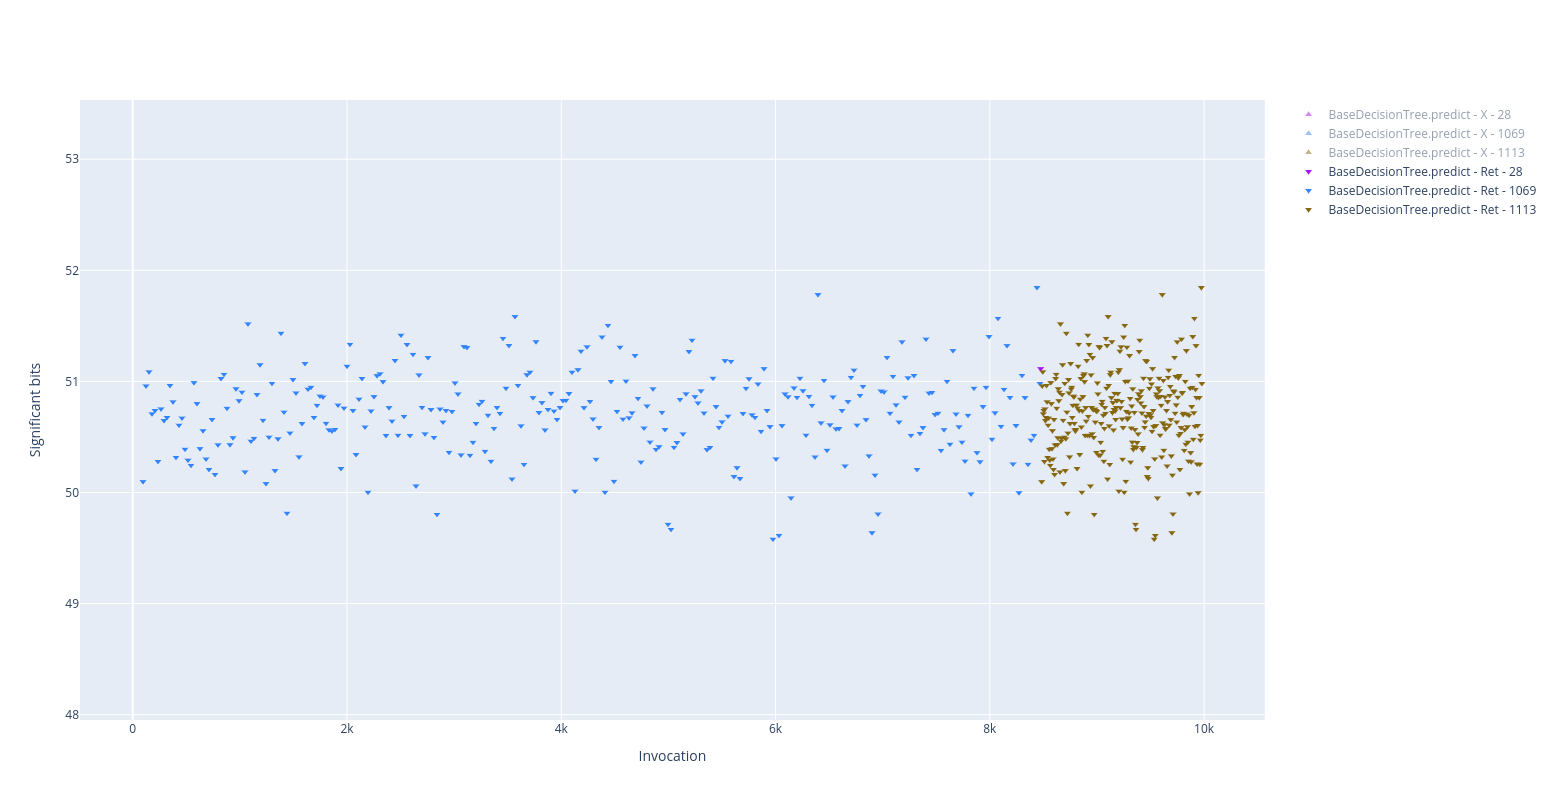
\includegraphics[width=\linewidth]{figure/adaboost/predict_adaboost_s.png}
    \caption{Number of significant digits of predicted values array.}
    \label{fig:adaboost_predict_s}
\end{figure}

\begin{figure}
    \centering
    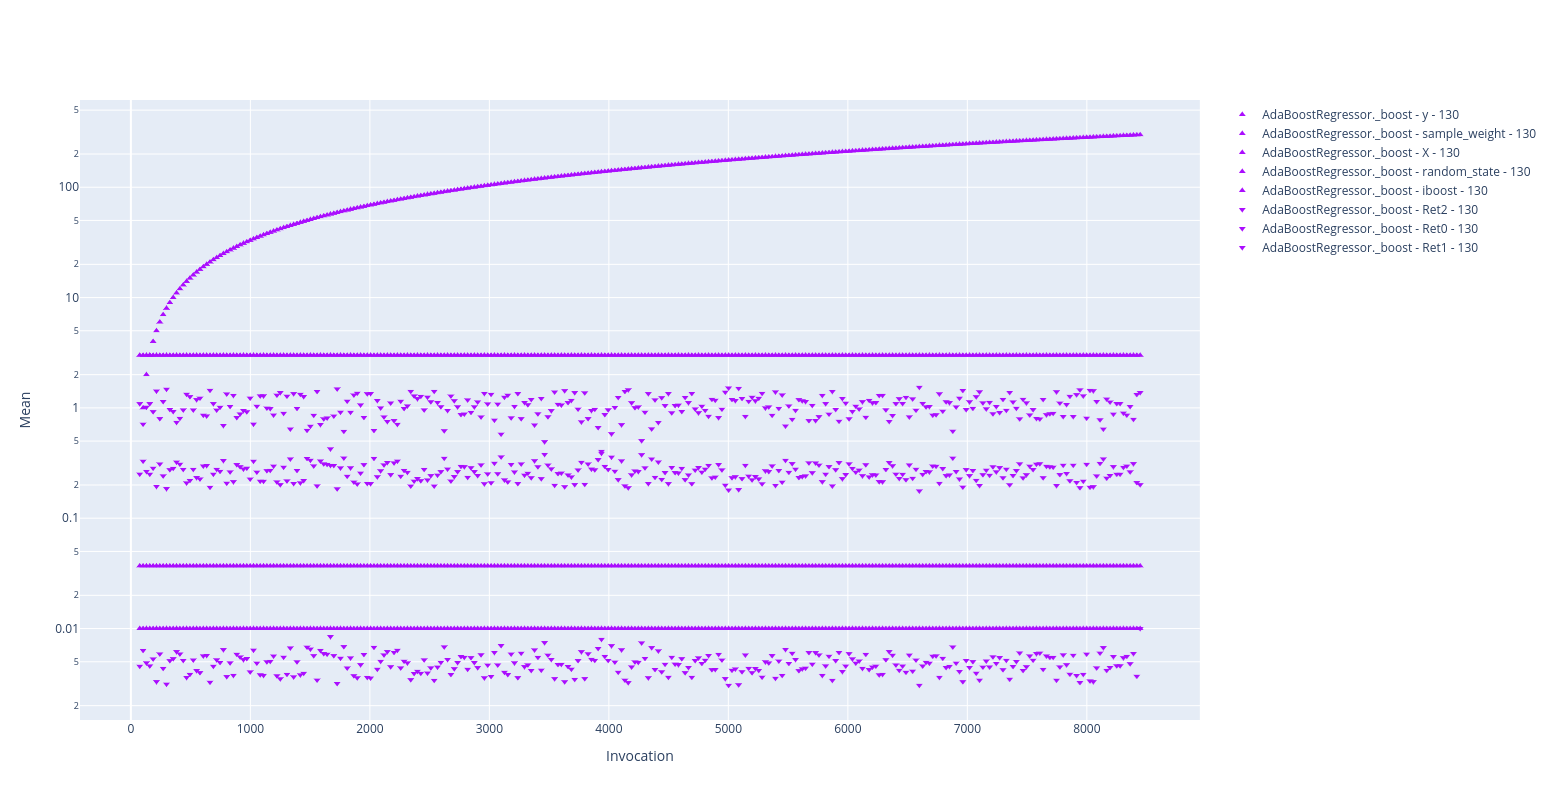
\includegraphics[width=\linewidth]{figure/adaboost/adaboost_boost_mean.png}
    \caption{Mean values of boost function.}
    \label{fig:adaboost_boost_mean}
\end{figure}

\begin{figure}
    \centering
    \caption{Caption}
    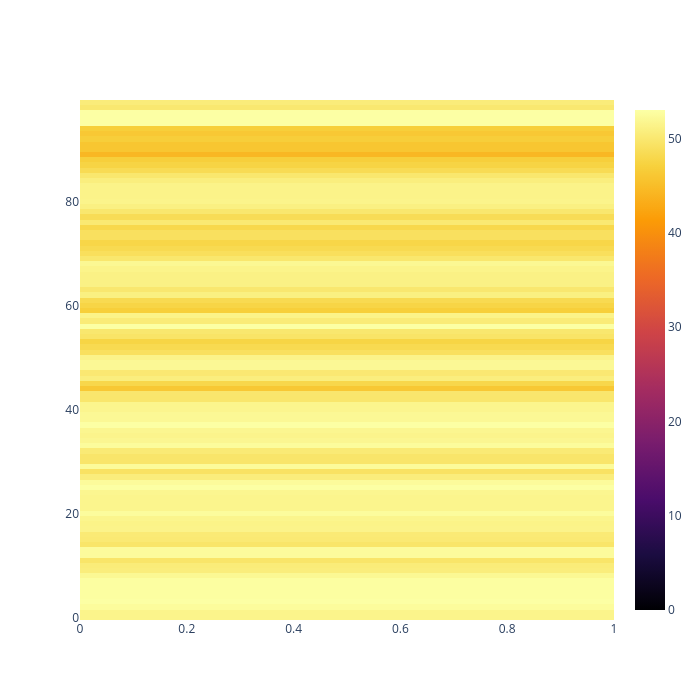
\includegraphics[width=\linewidth]{figure/adaboost/predict_adaboost_zoom_s.png}
    \caption{Average number of significant digits of prediction over estimator}
    \label{fig:adaboost_predict_zoom_s}
\end{figure}

\begin{figure}
\begin{minipage}{0.4\linewidth}
    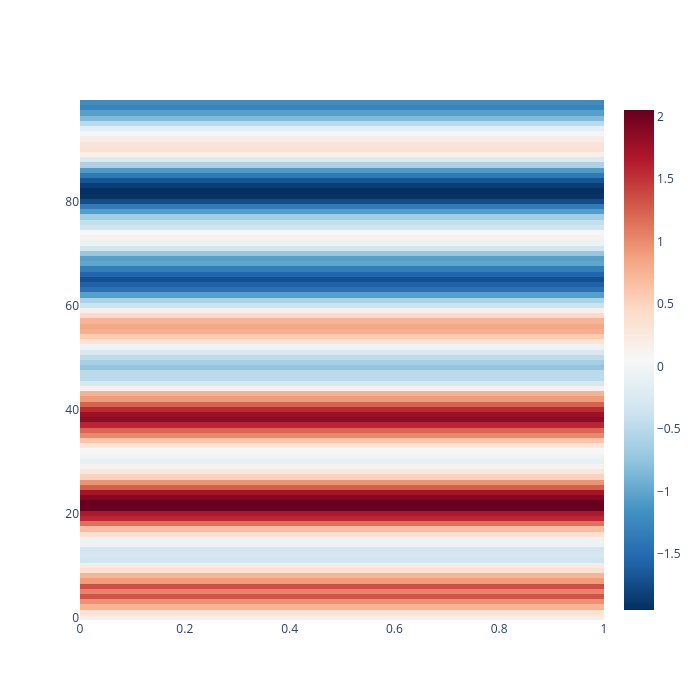
\includegraphics[width=\linewidth]{figure/adaboost/to_predict_adaboost_mean.png}
    \caption{Values to predict}
    \label{fig:adaboost_to_predict_mean}
\end{minipage}
\begin{minipage}{0.4\linewidth}
    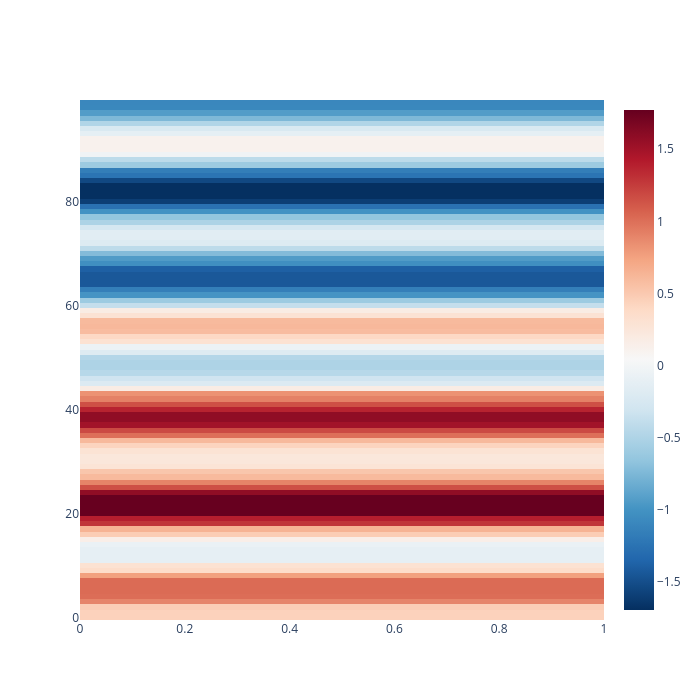
\includegraphics[width=\linewidth]{figure/adaboost/predict_adaboost_zoom_mean.png}
    \caption{Predicted values}
    \label{fig:adaboost_predicted_mean}
\end{minipage}
\caption{Comparison between original (fig.~\ref{fig:adaboost_to_predict_mean}) and predicted (fig.~\ref{fig:adaboost_predicted_mean}) values}
\end{figure}

\subsubsection{Bayesian Ridge Regression}

"\texttt{BayesianRidge} estimates a probabilistic model of the regression problem as described above. 
The prior for the coefficient  is given by a spherical Gaussian:
\[
    p(w|\lambda)=\mathcal{N}(w|0,\lambda^{-1}\mathbf{I}_p)
\]
The priors over  and  are chosen to be gamma distributions, the conjugate prior for the precision of the Gaussian. 
The resulting model is called Bayesian Ridge Regression, and is similar to the classical Ridge.
The parameters, and are estimated jointly during the fit of the model, 
the regularization parameters and being estimated by maximizing the log marginal likelihood. 
The scikit-learn implementation is based on the algorithm~\cite{tipping2001sparse}."

Both execution with RR and MCA modes failed but two different errors. 
Execution in RR mode raises an error due to an invalid value encountered in the \texttt{sqrt} function
while the MCA mode execution raises an error due to an issue with the Singular Value Decomposition (SVD) divergence.

RR executions fail with an invalid value in the \texttt{sqrt} function 
used in the \texttt{\_update\_coef\_} method of the \texttt{BayesianRidge} class.
This method updates the posterior mean and compute the corresponding Root-Mean-Square-Error (rmse).

When we backtrack the error propagation, we see that 

MCA executions show the limit of Pytracer since the SVD decomposition in scipy is a wrapper around the 
\texttt{gesdd} or \texttt{gesvd} LAPACK~\cite{anderson1999lapack} functions. 
Numerical instabilities that are coming from this kernel are opaque for Pytracer since it works 
at the Python level. Tools working on C/FORTAN codes 
like Veritracer~\cite{chatelain2018veritracer} can be used to zoom in on these functions.
Nevertheless, Pytracer provides have a visualization of the input used by the SVD and several
metrics used in numerical analysis, like the condition number, that can help to understand.

\subsection{Classifier comparisions}

This test compares the performance of 6 online solvers on the hand-written digits dataset.
These 6 solvers are:
\begin{itemize}
    \item Stochastic Gradient Descent 
    \item Averaged Stochastic Gradient Decent
    \item Perceptron
    \item Passive-Aggressive I \& II
    \item SAG: Minimizing Finite Sums with the Stochastic Average Gradient
\end{itemize}

Each solver is trained and predicts 20 times on 6 different training size ratio.

Figure~\ref{fig:classifier_comparisons_general} shows the all functions
traced by Pytracer over time. We can see the estimated number of significant digits varies a lot between 
values from 1 to 80 bits. Figure~\ref{fig:classifier_comparisons_mean_predictions} shows 
the average prediction score for each classifiers. The yellow points 
represent the average correct prediction score for one round and one classifier (line. 48) while blue points
tshows average predictions over the 20 rounds (line. 49).
We can see that precision is pretty low with an average solution below 10 significant bits, with 
an exception for values between the 24k and 32k invocation that correspond to the Perceptron
classifier. Indeed, this classifier is pretty stable with an average number of significant digits around 52 bits.


\begin{figure}
    \begin{lstlisting}[language=Python,style=customPython,numbers=left, firstnumber=19]
    heldout = [0.95, 0.90, 0.75, 0.50, 0.01]
    rounds = 20
    X, y = datasets.load_digits(return_X_y=True)

    classifiers = [
        ("SGD", SGDClassifier(max_iter=100)),
        ("ASGD", SGDClassifier(average=True)),
        ("Perceptron", Perceptron()),
        ("Passive-Aggressive I", PassiveAggressiveClassifier(loss='hinge',
                                                             C=1.0, tol=1e-4)),
        ("Passive-Aggressive II", PassiveAggressiveClassifier(loss='squared_hinge',
                                                              C=1.0, tol=1e-4)),
        ("SAG", LogisticRegression(
            solver='sag', tol=1e-1, C=1.e4 / X.shape[0]))
    ]

    xx = 1. - np.array(heldout)

    for name, clf in classifiers:
        print("training %s" % name)
        rng = np.random.RandomState(42)
        yy = []
        for i in heldout:
            yy_ = []
            for r in range(rounds):
                X_train, X_test, y_train, y_test = \
                    train_test_split(X, y, test_size=i, random_state=rng)
                clf.fit(X_train, y_train)
                y_pred = clf.predict(X_test)
                yy_.append(1 - np.mean(y_pred == y_test))
            yy.append(np.mean(yy_))
        plt.plot(xx, yy, label=name)
    \end{lstlisting}
    \label{fig:wrapper_code}
\caption{Illustration of the issue of using \texttt{frompyfunc} function to convert function to \texttt{ufunc}.}
\end{figure}




\begin{figure}
    \centering
    \caption{Caption}
    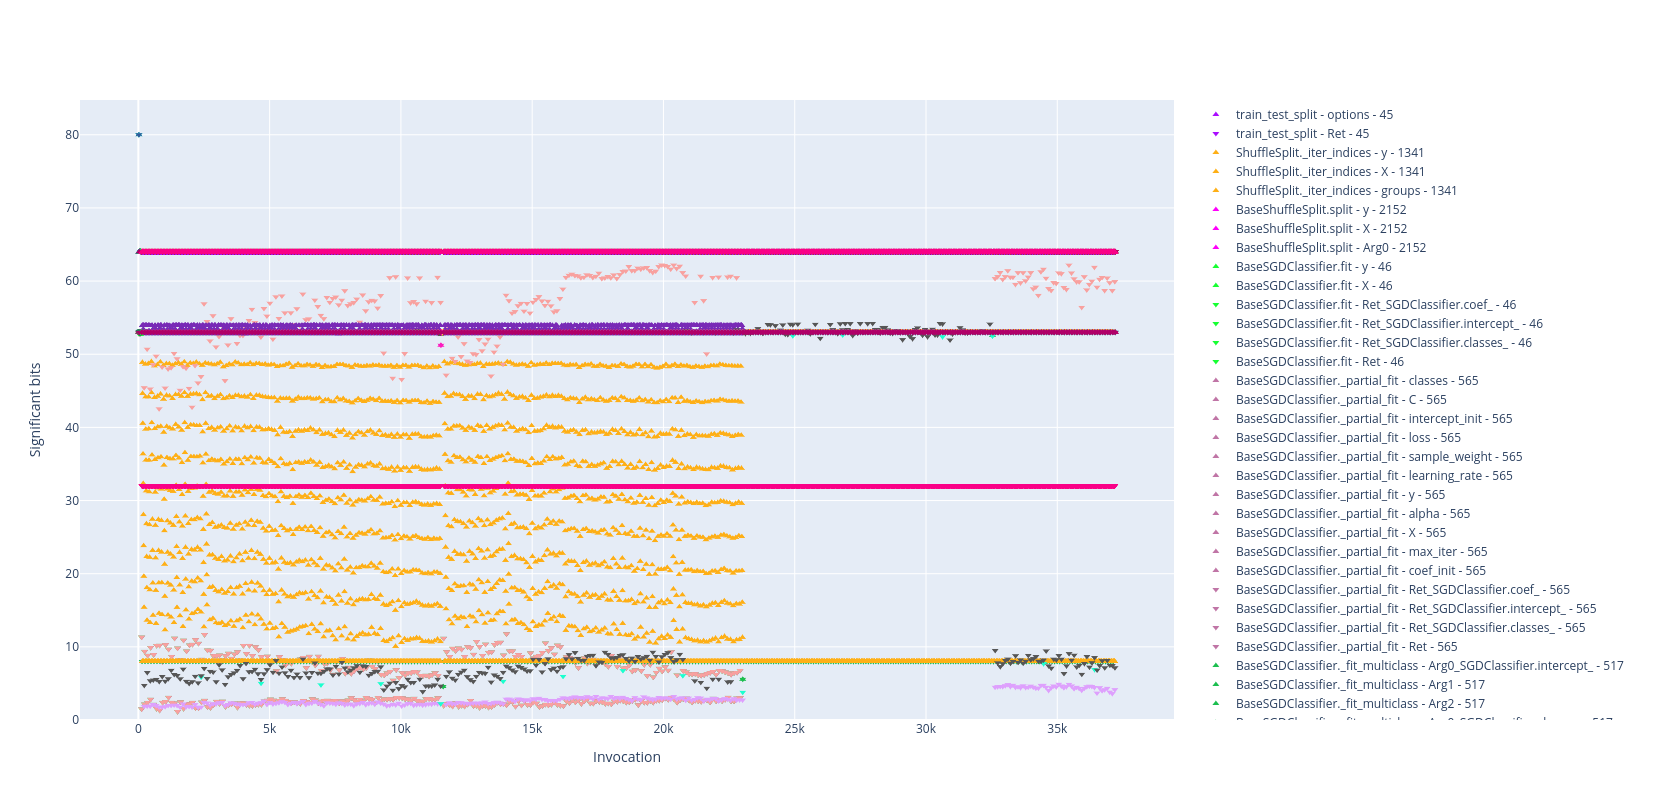
\includegraphics[width=\linewidth]{figure/classifier_comparisons/general.png}
    \caption{Number of significant digits (General view).}
    \label{fig:classifier_comparisons_general}
\end{figure}

\begin{figure}
    \centering
    \caption{Caption}
    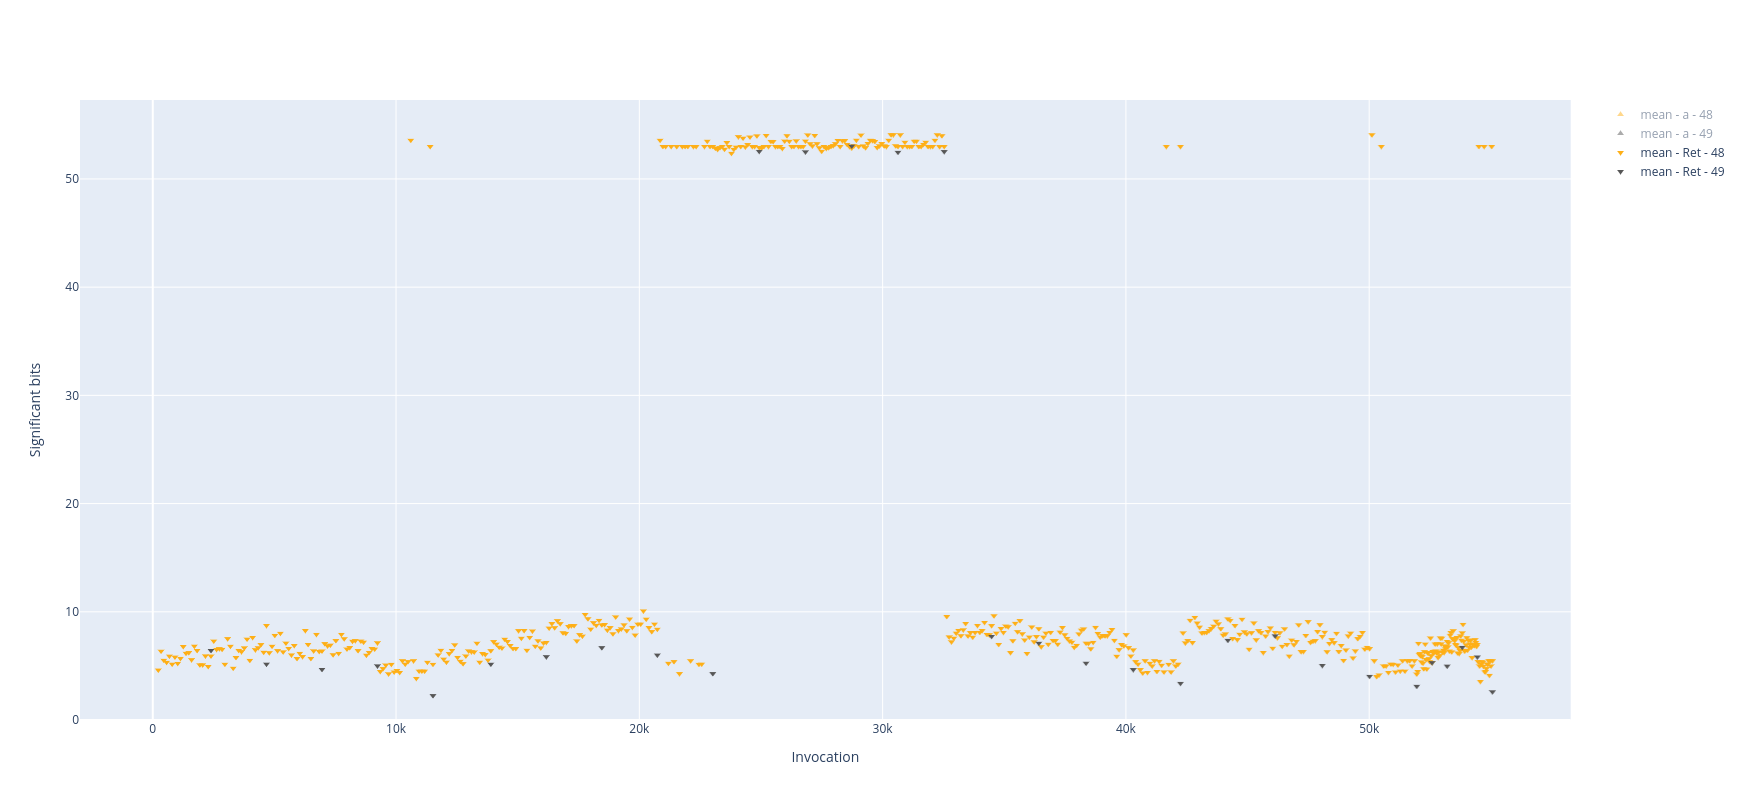
\includegraphics[width=\linewidth]{figure/classifier_comparisons/mean_predicition_s.png}
    \caption{Number of significant digits (General view).}
    \label{fig:classifier_comparisons_mean_predictions}
\end{figure}

\begin{figure}
    \centering
    \caption{Caption}
    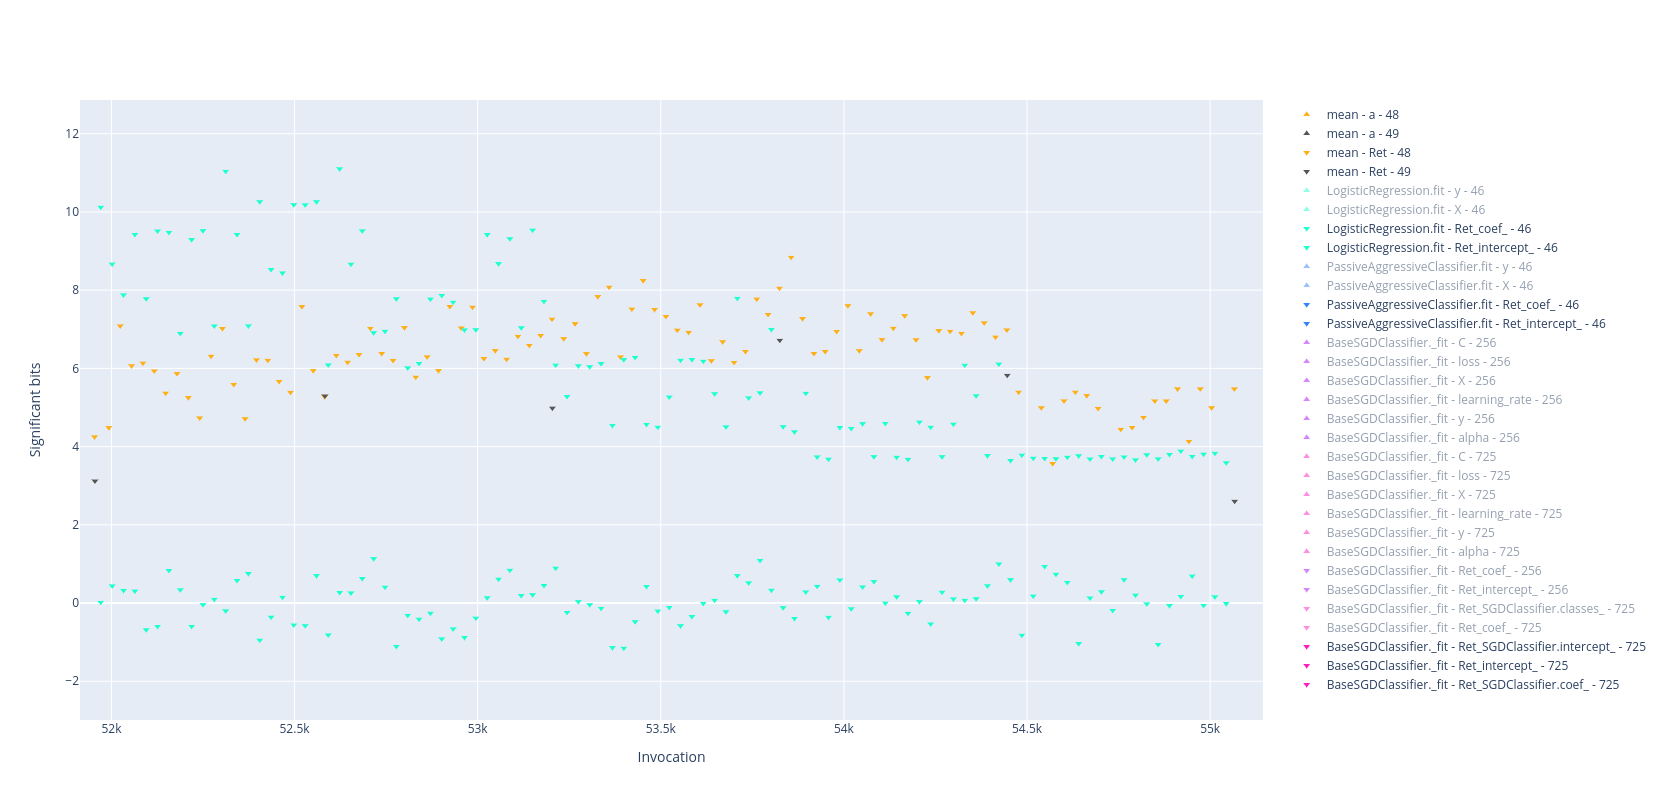
\includegraphics[width=\linewidth]{figure/classifier_comparisons/SAG_predicition_s.png}
    \caption{Number of significant digits (General view).}
    \label{fig:classifier_comparisons_general}
\end{figure}

\begin{figure}
    \centering
    \caption{Caption}
    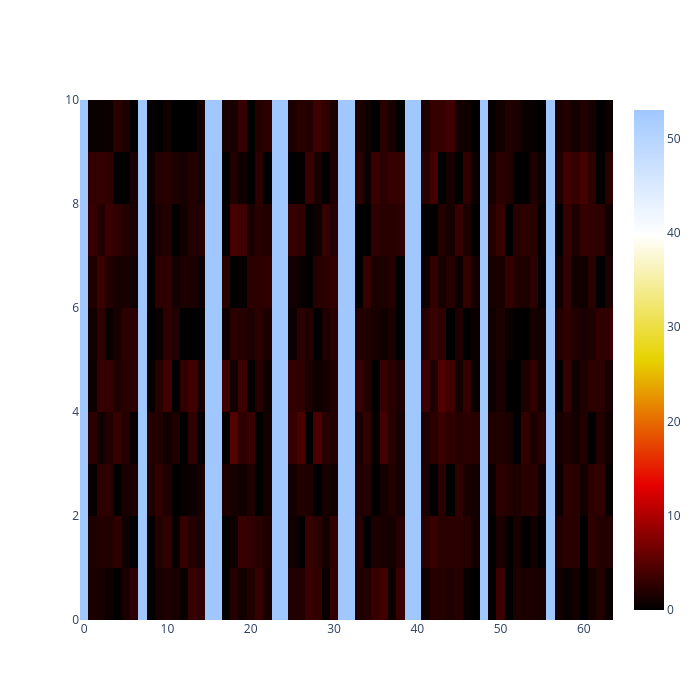
\includegraphics[width=\linewidth]{figure/classifier_comparisons/zoom_SAG_fit_coef_s.png}
    \caption{Number of significant digits (General view).}
    \label{fig:classifier_comparisons_general}
\end{figure}


\subsection{Cluster IRIS}


\begin{figure}
    \centering
    \caption{Caption}
    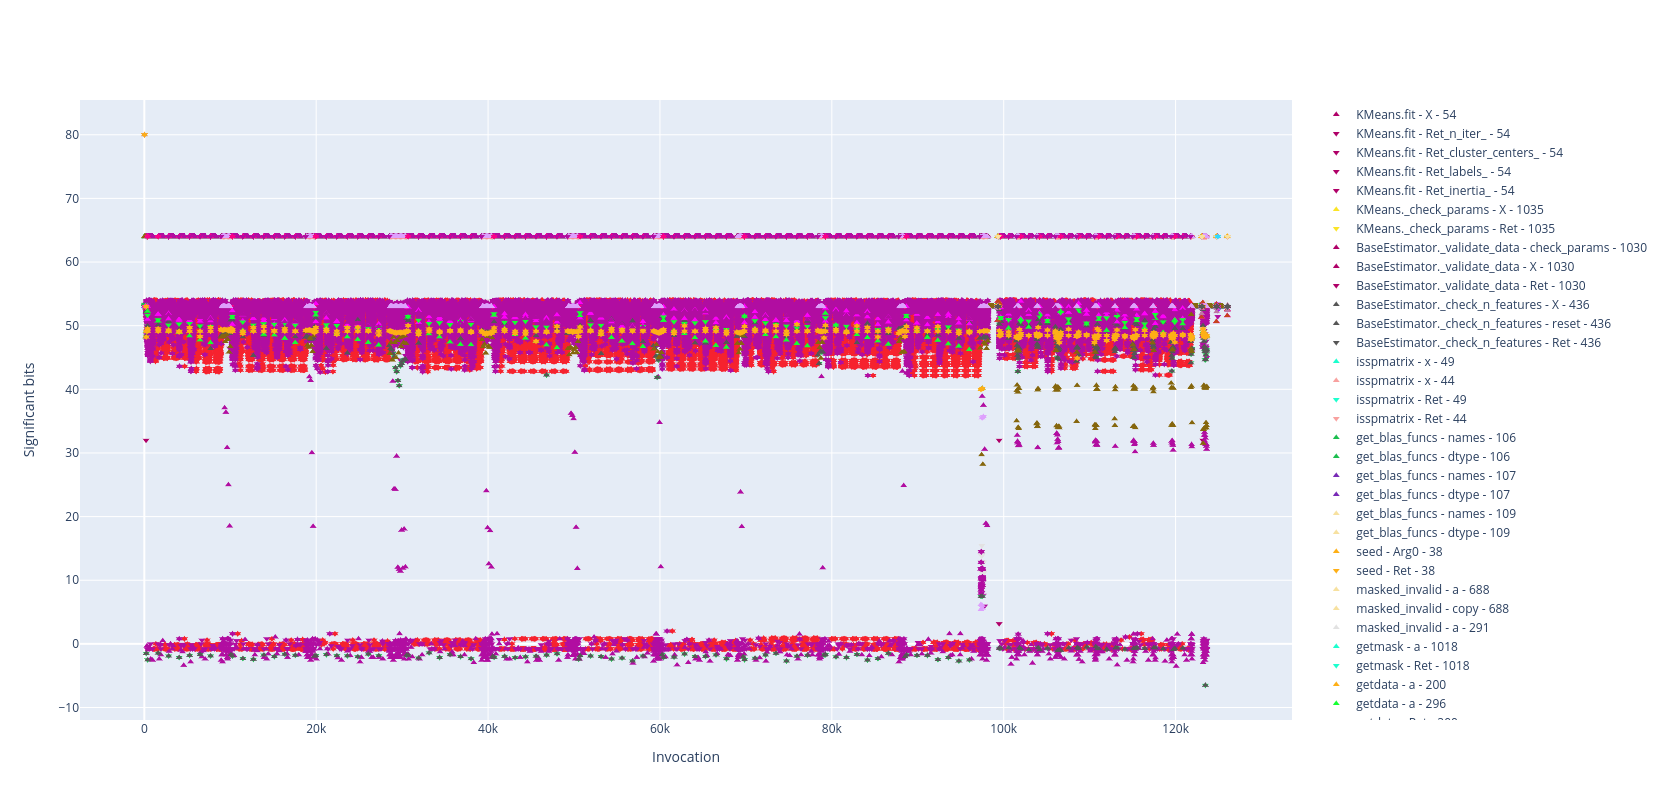
\includegraphics[width=\linewidth]{figure/cluster_iris/general.png}
    \caption{Number of significant digits (General view).}
    \label{fig:cluster_iris_general}
\end{figure}


\subsection{PyAFQ}


PyAFQ is Python package for Automated Fiber Quantification.
It aims at finding delineation of the major fiber tracts in individual human brains, and quantification of the tissue properties within the tracts.

\section{Performance evaluation}

In this section, we review the performance overhead of the Pytracer's instrumentation cost
and the time spent during the postprocessing analysis. 

\subsection{Overhead}

Pytracer instrumentation overhead comes from the time spent to instrument module (initialization overhead)
before executing the targeted application plus the cost for dumping the data during the execution (running overhead).
However, initialization overhead is amortized when traced applications are above ....
Table~\ref{tab:pytracer_overhead} summaries the slowdown measure on pyAFQ test.
We can see that Pytracer only a gives reasonable slowdown of $\times 6$.

\begin{table}[]
    \centering
    \begin{tabular}{c|c|c|c|c}
         Pytracer & Verificarlo Instrumentation & Backend & Time (hours:minutes:seconds) & Overhead \\
         \hline 
         No & No & - & 00:30:51 & 1 \\
         No & Yes & IEEE & 01:32:56 & 3 \\
         No & Yes & RR & 16:52:08 & 32 \\
         Yes & No & - & 03:11:07 & 6  \\
         Yes & Yes & IEEE & 11:14:33 & 22 \\
         Yes & Yes & RR & 25:05:54 & 48 \\
    \end{tabular}
    \caption{Caption}
    \label{tab:pytracer_overhead}
\end{table}

% \begin{table}[]
%     \centering
%     \begin{tabular}{c|c|c|c|c}
%          Pytracer & Verificarlo Instrumentation & Backend & Time (hours:minutes:seconds) & Overhead \\
%          \hline 
%          No & No & - & 15 & 1 \\
%          No & Yes & IEEE & 49 & 3 \\
%          No & Yes & RR &  & 441 & 29 \\
%          Yes & No & - & 03:11:07 & 6  \\
%          Yes & Yes & IEEE & 11:14:33 & 22 \\
%          Yes & Yes & RR & 25:05:54 & 48 \\
%     \end{tabular}
%     \caption{Caption}
%     \label{tab:pytracer_overhead}
% \end{table}

\subsection{Postprocessing}




\section{Discussion}

\begin{itemize}
    \item Control flow divergence
    \item MCA mode -> semantic bugs
    \item Pytracer is flexible and works with any type of perturbations (uncertainty quantification, internal randomness, parallel sections).

\end{itemize}

\section{Conclusion}

\bibliographystyle{abbrv}
\bibliography{biblio}

%%
%% If your work has an appendix, this is the place to put it.
\appendix

\end{document}
\endinput
%%
%% End of file `sample-authordraft.tex'.
